\documentclass[11pt]{article}
\usepackage[margin=1in]{geometry}
\usepackage{mathpazo}
\usepackage{amsmath,amssymb,amsthm}
\usepackage[expansion=false]{microtype}
\usepackage{xcolor}
\usepackage{booktabs,tabularx,array,longtable}
\usepackage{enumitem}
\usepackage{listings}
\usepackage{graphicx}
\usepackage{tikz}
\usetikzlibrary{positioning,arrows.meta,fit,calc,backgrounds}
\usepackage{xurl}
\usepackage[hidelinks]{hyperref}

\theoremstyle{definition}
\newtheorem{requirement}{Requirement}
\newtheorem{principle}{Principle}
\newtheorem{decision}{Open decision}
\newtheorem{obligation}{Obligation}
\newtheorem{finding}{Finding}
\newtheorem{workpackage}{Work package}
\theoremstyle{remark}
\newtheorem{remark}{Remark}

\newcommand{\MUST}{\textsc{must}}
\newcommand{\MUSTNOT}{\textsc{must not}}
\newcommand{\SHOULD}{\textsc{should}}
\newcommand{\SHOULDNOT}{\textsc{should not}}
\newcommand{\MAY}{\textsc{may}}
\usepackage[htt]{hyphenat}
\newcommand{\code}[1]{\texttt{#1}}
\newcommand{\Gz}{F1R3Gaze}
\newcommand{\Hr}{ign1t10n}
\newcommand{\Nd}{F1R3Node-Rust}
\newcommand{\Camp}{CampF1R3}
\newcommand{\Gm}{F1R3Games}
\newcommand{\Svc}{\code{f1r3games-service}}
\newcommand{\Em}{Embers}
\setlength{\emergencystretch}{3em}

\definecolor{cm}{RGB}{90,110,90}
\definecolor{newbg}{RGB}{255,248,214}
\lstset{
  basicstyle=\ttfamily\small,
  commentstyle=\color{cm}\itshape,
  columns=fullflexible,
  keepspaces=true,
  frame=single,
  framerule=0.3pt,
  rulecolor=\color{black!30},
  xleftmargin=4pt,xrightmargin=4pt,
  aboveskip=6pt,belowskip=6pt,
  breaklines=true,
  upquote=true
}
\lstdefinelanguage{Hocon}{comment=[l]{\#}, morestring=[b]"}
\lstdefinelanguage{Conf}{comment=[l]{\#}}

\title{\textbf{ign1t10n: macOS Installer Specification}\\[4pt]
\large One install: a multi-validator \Nd{} shard, its observer, the \Gz{} browser,\\
and the \Gm{} portal and games, served to any web browser\\[6pt]
\normalsize Version 0.4 (draft for review)}
\author{Lucius Gregory Meredith\\
\small CEO, F1R3FLY.io, and Chief Science Officer, F1R3FLY Industries}
\date{7 October 2026}

\begin{document}
\maketitle

\begin{abstract}
\noindent
This specification defines \Hr{}, an installer for macOS that leaves a person, a
few minutes after double-clicking one file, with a working \Nd{} shard on their own
machine (a bootstrap node, two to ten validators, and a read-only observer), the
\Gz{} browser configured to deploy to that shard and read from it, and, new in this
version, the \Gm{} portal and its games, installed on the shard and served on
\code{http://localhost} so that an ordinary web browser (Safari, Chrome, Firefox) can
sign on, launch new game instances, play them, and browse each game's gallery of
plays. The portal is \Svc{}, the Rust service of the \Gm{} repository, supervised by
\Hr{} as one more process beside the nodes and \Em{}; each game client is served from
an origin of its own, as the portal's frame model requires. Installation of the games
on the chain (the portal's environment, each game's environment, and the
registration of the games by a local stand-in for the F1R3FLY.io Cooperative) is
automated, resumable and recorded in the manifest, replacing the eleven manual steps
the first live installs of 5 and 6 October needed.

The specification is grounded in \Hr{} \code{main} at \code{46faa56} (the first
working implementation of version 0.3), \Gm{} at \code{57a3b27} (branch
\code{f1r3beat}, the portal with F1R3Pix and F1R3Beat), \Nd{} at \code{fce422a},
\Gz{} at \code{f6ee26a}, and the \Gm{} portal, F1R3Pix and F1R3Beat design documents.
\end{abstract}

\tableofcontents
\newpage

%======================================================================
\section{What changed in version 0.4}\label{sec:changes}

\begin{enumerate}[itemsep=2pt]
\item \textbf{\Gm{} is a component of the install} (default on, like \Em{}): the
  portal service, the F1R3Pix and F1R3Beat web clients, the games' environments on
  the shard, their registration, and a ``F1R3Games'' item in the menu bar that opens
  the portal in the person's default browser. New: Findings~\ref{f:svc}--\ref{f:gazejs},
  Principles~\ref{p:origin}--\ref{p:keys}, \S\ref{sec:games} (the component),
  stages G1--G7 (\S\ref{sec:gstages}), work packages F1--F7 in the \Gm{} repository
  (\S\ref{sec:fwp}) and H7--H9, R2, T2 here, acceptance tests A15--A23, and
  decisions~\ref{dec:ports}--\ref{dec:default}.
\item \textbf{The decisions of 30 September are folded in} (\S\ref{sec:resolved}):
  the separate bootstrap is kept; Apple silicon only; macOS 13.0 minimum;
  10\,000\,000~F1R3 to the browser's wallet; deploys go to a randomly selected active
  validator; timings tuned for a laptop; the node refuses HTTP requests carrying a
  foreign \code{Origin} (N5); \Em{} is an installation option, default on.
\item \textbf{What the first working build taught is adopted as specification}
  (from \code{docs/IMPLEMENTATION.md} at \code{46faa56}): the supervisor is a classic
  per-user launch agent loaded with \code{launchctl bootstrap}, not an
  \code{SMAppService} agent; the genesis ceremony waits for $N_0 - 1$ approvals; all
  six ports and the network id go on each node's command line; the bootstrap's node
  id is read from its output; node logs go to standard output; templates are compiled
  into the binary; the archive is \code{macos-arm64}.
\end{enumerate}

%======================================================================
\section{Scope and conventions}\label{sec:scope}

\subsection{What the installer delivers}

After a successful install on a supported Mac, with no further action beyond
approving a background item in System Settings when macOS asks:

\begin{enumerate}[nosep]
\item \code{/Applications/F1R3Gaze.app} and \code{/Applications/ign1t10n.app} are
  installed, signed and notarised.
\item A per-user launch agent, \code{io.f1r3fly.ign1t10n.supervisor}, is loaded and
  running. It supervises:
  \begin{itemize}[nosep]
  \item a \emph{bootstrap} node, which coordinated the genesis ceremony and is every
    other node's rendezvous; it is not bonded and never proposes;
  \item $N$ \emph{validators}, bonded at genesis or by a later resize, which propose
    and finalise blocks ($N = 2$ unless the person chose otherwise, $2 \le N \le 10$);
  \item one \emph{observer}, a read-only node that serves every read;
  \item \Em{}, unless the person turned it off;
  \item the \emph{portal}, \Svc{}, unless the person turned \Gm{} off.
  \end{itemize}
\item Every key was generated on this machine at install time. The shard's genesis
  funds the person's active \Gz{} wallet and a local faucet; the faucet funds \Em{},
  the portal and the local Cooperative.
\item \Gz{} deploys to a randomly selected active validator, reads from the observer,
  and is open in a window.
\item The \Gm{} portal environment and the five game environments are installed on
  the shard; F1R3Pix and F1R3Beat are registered; the portal answers at
  \code{http://localhost:40700} and has been opened in the default browser, where the
  person can create a keystore, be funded by the faucet, launch a game, and browse its
  gallery.
\item Every listening socket of every supervised process is bound to a loopback
  address.
\item The shard and the portal survive logout, sleep and reboot, and come back with
  the chain, the portal's origin and every browser keystore intact, at the size last
  chosen.
\end{enumerate}

\noindent
Throughout, ``$N$ nodes'' in the user interface means $N$ validators; the bootstrap
and the observer are always present and are shown separately. With the defaults,
five \code{f1r3node} processes, \Em{} and the portal run.

\subsection{Non-goals for this version}

More than ten validators; joining a remote or public shard; exposing the local shard
or the portal to the network (so invitations work for other browsers and other
accounts on this Mac only); stake other than equal stakes; Intel Macs, Linux and
Windows; Docker; running the \Gm{} portal \emph{inside} \Gz{} (it executes no
JavaScript; \S\ref{sec:gazerendition}); web clients for F1R3Ink, F1R3SideChat and
F1R3Skein, which do not exist yet; the F1R3Skein visionOS instrument.

\subsection{Pinned baselines}

\begin{center}\small
\renewcommand{\arraystretch}{1.15}
\begin{tabularx}{\linewidth}{@{}p{2.6cm}p{3.0cm}X@{}}
\toprule
Source & Revision & Notes\\
\midrule
\Hr{} & \code{main} @ \code{46faa56} & ``first working version'' of v0.3; \code{docs/IMPLEMENTATION.md} records its decisions, deviations and known issues\\
\Nd{} & \code{master} @ \code{fce422a} & crate \code{node} v0.4.46; toolchain \code{nightly-2026-02-09}; topology reference \code{docker/shard.yml}\\
\Gz{} & \code{main} @ \code{f6ee26a} & release v0.1.0; crates \code{gaze-shard}, \code{gaze-wallet} reused by \Hr{}; renders HTML with Blitz and runs no JavaScript\\
\Em{} & \code{28e50d4} & bundled as \code{Helpers/embers}; its contracts do not parse on \code{fce422a} (known issue)\\
\Gm{} & \code{f1r3beat} @ \code{57a3b27} & \code{Portal/f1r3games-portal} (Rust workspace: \code{core}, \code{wallet}, \code{node}, \code{service}, \code{cli}, \code{games}, \code{rholint}; React shell in \code{web/}); \code{F1R3Pix/client}, \code{F1R3Beat/client}; to be re-pinned to \code{main} once merged\\
Designs & 5--6 October 2026 & \Gm{} Portal design v0.1; F1R3Pix design v1; F1R3Beat design v2\\
\bottomrule
\end{tabularx}
\end{center}

\subsection{Conventions}

\MUST, \MUSTNOT, \SHOULD, \SHOULDNOT{} and \MAY{} carry their RFC 2119 meanings.
``The state directory'' is \code{\textasciitilde/Library/Application Support/F1R3FLY/ign1t10n}.
``The profile'' is \Gz{}'s profile directory. ``The portal'' is the running \Svc{}
process together with the web shell it serves; ``the portal environment'' is the
\code{games} environment it installs on the shard; ``a game environment'' is one
game's contract. ``The local Cooperative'' is a key \Hr{} generates to stand in for
the F1R3FLY.io Cooperative on this shard (Decision~\ref{dec:coop}). ``An origin''
is a scheme, host and port, as browsers define it. Ports are written for the default
allocation.

%======================================================================
\section{Findings}\label{sec:findings}

These are the facts the design rests on. Findings~\ref{f:readonly}--\ref{f:lifecycle}
are carried from version 0.3, shortened where the implementation has since settled
them; Findings~\ref{f:svc}--\ref{f:gazejs} are new.

\subsection{The shard}

\begin{finding}[The observer is not optional]\label{f:readonly}
Every endpoint that runs an exploratory deploy is served only by read-only nodes; a
validator answers \code{400 readonly\_node\_required}. That covers
\code{POST /api/explore-deploy}, \code{POST /api/estimate-cost},
\code{GET /api/registry/\{uri\}} and \code{GET /api/balance/\{address\}}
(\code{docs/node/api-reference.md}). \Gz{}, \Em{} and \Svc{} all read there.
\end{finding}

\begin{finding}[The tested topology]\label{f:topology}
\code{docker/shard.yml} runs a bootstrap started with \code{--ceremony-master-mode},
\code{--required-signatures} and \code{--heartbeat-disabled}, absent from
\code{bonds.txt}; genesis validators started with \code{--genesis-validator} and
\code{--bootstrap} pointing at it; and an observer bootstrapping from it. \Hr{} runs
that shape on loopback, generalised from three validators to $N$.
\end{finding}

\begin{finding}[Same host, distinct ports]\label{f:loopback}
On one Mac every node advertises \code{127.0.0.1} and differs by port. The node's
port options have default values that override the configuration file, so all six
ports go on the command line; the outgoing network id defaults to \code{testnet}
unless \code{--network-id} is given (both found on the first real multi-node run).
\end{finding}

\begin{finding}[Approvals]\label{f:approvals}
The node requires strictly fewer ceremony approvals than genesis validators;
\code{shard.yml} uses 2 of 3. \Hr{} passes $\max(N_0 - 1, 1)$.
\end{finding}

\begin{finding}[The shard can be resized while running]\label{f:resize}
A node that was not at genesis joins by last-finalised-state fetch, is funded,
submits a bond deploy to a \emph{bonded} validator, and becomes active at the next
epoch boundary (\code{docs/node/joining-a-network.md}); leaving is
\code{PoS!("withdraw", ...)}, effective at the next boundary, with payout after the
quarantine. \code{epoch-length} and \code{quarantine-length} are 10, so both take
seconds to minutes locally. A bonded validator that does not propose is counted in
consensus while contributing nothing.
\end{finding}

\begin{finding}[Deploys can be signed outside the node]\label{f:signing}
\Gz{}'s \code{gaze-shard} produces deploys byte for byte as the node verifies them;
\code{gaze-wallet} renders the vault transfer. \Hr{} uses both for faucet transfers,
bond, withdraw and sweep deploys.
\end{finding}

\begin{finding}[The shipped development keys are public]\label{f:devkey}
\code{docker/.env.example} and the committed \code{docker/.env} carry the private
keys of every node in the Docker topologies and control the genesis supply there.
The \Gm{} repository likewise commits example keys under
\code{Portal/f1r3games-portal/examples/local-shard/} (a service key, an environment
key, a token secret and five game environment keys). No install may reuse any of
them.
\end{finding}

\begin{finding}[How a key can reach a process]\label{f:keypath}
\code{--validator-private-key} exposes the key in the argument vector;
\code{--validator-private-key-path} takes an encrypted PEM whose password comes from
\code{F1R3NODE\_VALIDATOR\_PASSWORD}. \Svc{} reads its keys only from plaintext
key files named in its configuration (\code{service\_key\_file},
\code{env\_key\_file}, \code{token\_secret\_file}) and the game keys from a
directory (\code{--keys}); it reads them once, at start.
\end{finding}

\begin{finding}[Bind addresses and origins]\label{f:bind}
\code{api-server.host} is configurable; the protocol transport and discovery bind
\code{0.0.0.0} until N1 lands. With N5, the node answers 403 to any HTTP request
carrying an \code{Origin} header, so no page in a stock browser can use a local node
directly; programs that send no \code{Origin} (\Gz{}, \Em{}, \Svc{}) are unaffected.
\end{finding}

\begin{finding}[Lifecycle facts]\label{f:lifecycle}
The node handles \code{SIGTERM}. A joined node restarted on the same data directory
reconnects in about a second; its identity is the TLS certificate in the data
directory, so a data directory must never be deleted while peers remember it. During
the ceremony the bootstrap cannot answer \code{/api/status}; its node id is read from
what it prints at start.
\end{finding}

\subsection{\Gm{}}

\begin{finding}[The portal is one Rust service]\label{f:svc}
\Svc{} (crate \code{f1r3games-service}, axum) serves the API under \code{/api} and,
as a fallback service, the built React shell from \code{static\_dir}, on the single
address in \code{listen} (default \code{127.0.0.1:8640}). It holds three secrets:
the \emph{service key}, which pays the environment deploys and the testnet faucet;
the \emph{environment key}, which signs the portal environment's
\code{insertSigned} registration and so fixes its registry URI; and a \emph{token
secret}. It deploys to one \code{validator\_url} and reads at one
\code{observer\_url}; it never proposes (validators propose by heartbeat, which
\Hr{} leaves on). Subcommands: \code{serve} (default; installs the environment first
when \code{bootstrap\_env} is true), \code{bootstrap}, \code{env-uri},
\code{keygen}, \code{games-keygen}, \code{games-install --keys DIR --version V},
\code{games-manifests --keys DIR --entry-base URL --out FILE}. The portal design
placed this logic in an \Em{} domain; the implementation chose a dedicated service,
and the implementation governs here: \Gm{} does not need \Em{}.
\end{finding}

\begin{finding}[The browser never reaches the node]\label{f:nonode}
The shell's wallet is Rust compiled to WebAssembly (\code{crates/wallet}); it signs in
the page and hands signed deploys to \Svc{} (\code{/api/prepare}, \code{/api/send});
reads go through \code{/api/explore} and the \code{GET} routes. The page holds no node
URL. N5 therefore stands without exception.
\end{finding}

\begin{finding}[Games run on origins of their own]\label{f:origins}
The portal frames a game in a sandboxed \code{iframe}
(\code{allow-scripts allow-same-origin allow-forms allow-pointer-lock
allow-downloads}) and answers its host protocol by \code{postMessage}, accepting
only messages whose \code{event.origin} is the origin of the game's registered
\code{entry} and whose source is that frame (\code{web/src/core/host.ts}).
\code{allow-same-origin} is safe only because the game is on another origin, and
\code{GameFrame.tsx} refuses to frame a game served from the portal's own origin.
A game client is a static Vite build (\code{base: "./"}) loaded as
\code{<entry>?instance=<id>\&portal=<origin>}; its gallery renderers are
\code{<entry>preview/<kind>.html}. F1R3Pix (renderer \code{canvas}) and F1R3Beat
(\code{pattern}, \code{session}) have clients; F1R3Ink and F1R3SideChat have only
environments; F1R3Skein's manifest lists \code{visionos} and \code{web} and has no web
client.
\end{finding}

\begin{finding}[Browser state belongs to an origin]\label{f:browserstate}
The keystore, contacts and the pinned environment URI live in IndexedDB under the
portal's origin (\code{web/src/core/store.ts}). A passkey is created with no explicit
relying-party id, so it is bound to the origin's host; WebAuthn refuses IP literals
as relying-party ids, and \code{localhost} is a secure context in Safari, Chrome and
Firefox. Hence the portal \MUST{} be reached as \code{http://localhost:}\textit{port},
and that origin \MUST{} not change for the life of the install: at
\code{127.0.0.1:}\textit{port}, or at another port, the person meets an empty
keystore and passkeys that do not work.
\end{finding}

\begin{finding}[Keys fix the environment URIs, and wallets pin them]\label{f:pin}
The portal environment's URI is derived from the environment key; each game
environment's URI from that game's key; every call template in a manifest embeds its
game's URI, so the manifest's template hashes depend on the keys. At sign-on the
shell pins the portal environment URI and afterwards refuses a service that serves
another (\code{web/src/core/portal.ts}). Rotating the environment key therefore
strands every keystore in every browser.
\end{finding}

\begin{finding}[Installation is an ordered sequence of deploys]\label{f:order}
On a new chain: fund the service key; install the portal environment (one deploy
of up to \code{env\_phlo\_limit}, 50\,M phlo by default) and wait until the
\code{env.probe} template reports the version; install each game environment
(\code{games-install}); write the manifests (\code{games-manifests}), which take a
single \code{--entry-base} and produce \code{<base>/<id>/}; register each with
\code{games.register}, which the environment accepts only from the
\code{coop\_address} that was rendered into it at install. Registration is today done
with the \code{f1r3games} CLI, which needs its own passphrase-protected keystore
holding the Cooperative's key (\code{register-games FILE [--only ID]}).
\end{finding}

\begin{finding}[Raising an environment's version discards its state]\label{f:upgrade}
Installing a higher \code{env\_version} of the portal environment re-initialises its
maps: profiles, instances, plays, invitations and sponsorships on that shard are not
carried over (\Gm{} \code{docs/IMPLEMENTATION.md}). Replacing a game environment's
body likewise replaces its per-instance state. A change to a game's call templates
changes the manifest hashes and requires re-registration; a change confined to a
web client changes nothing on chain.
\end{finding}

\begin{finding}[The faucet pays from the service key]\label{f:faucet}
\code{POST /api/testnet/fund} transfers \code{faucet.amount} dust (default
$10^8$, i.e.\ 1~F1R3) from the service key to an address the page names, when
\code{faucet.enabled}; the shell calls it during sign-on so a new key can pay for its
first deploy.
\end{finding}

\begin{finding}[What the first live installs needed by hand]\label{f:manual}
Standing the portal up on an \Hr{} shard on 5 and 6 October took: building the
service and shell (including \code{npm install --include=dev} and npm's install-script
approval for \code{esbuild}); \code{keygen} and \code{games-keygen}; reading the shard's
endpoints with \code{ctl env}; funding the service key and a stand-in Cooperative with
\code{ctl fund}; choosing a stand-in Cooperative address; editing
\code{f1r3games.toml}; \code{bootstrap} and waiting; \code{games-install};
\code{games-manifests}; importing the Cooperative key into the CLI and
\code{register-games}; and serving the game clients from a second development server
(\code{:5174}) so they had their own origin. Defects found only on the live shard
(the deploy-id parse, multi-line templates, \code{validAfterBlockNumber} from the
validator's sequence number, Nil dropped from tuples, escaped manifest sources,
\code{allow-same-origin}, \code{.contains} on lists, a \code{/\textbackslash\ List}
binder) are fixed at the pinned revision. Every manual step above becomes a stage of
\Hr{} (\S\ref{sec:gstages}); no developer tool is needed on the person's Mac.
\end{finding}

\begin{finding}[\code{localhost} has two addresses]\label{f:dualstack}
\code{localhost} resolves to \code{::1} and \code{127.0.0.1}, and browsers try both.
A service listening on one family leaves the other free for any program to bind, and
that program then answers some of the browser's requests: the same hazard version
0.3's implementation met with Docker's \code{*:p} listeners (\code{ports::port\_free}).
\end{finding}

\begin{finding}[\Gz{} runs no JavaScript]\label{f:gazejs}
\Gz{} renders HTML and CSS with Blitz and executes no JavaScript; behaviour is
f1r3lang. The React shell therefore runs only in a stock browser. The shell is cut so
that a later f1r3lang rendition can replace it (\code{docs/GAZE-MAPPING.md}); that
needs capabilities \Gz{} lacks today (allowances, \code{invite}, \code{open},
\code{pay}, \code{frame}, per-site storage).
\end{finding}

%======================================================================
\section{Architecture}\label{sec:arch}

\begin{figure}[htbp]
\centering
\resizebox{\linewidth}{!}{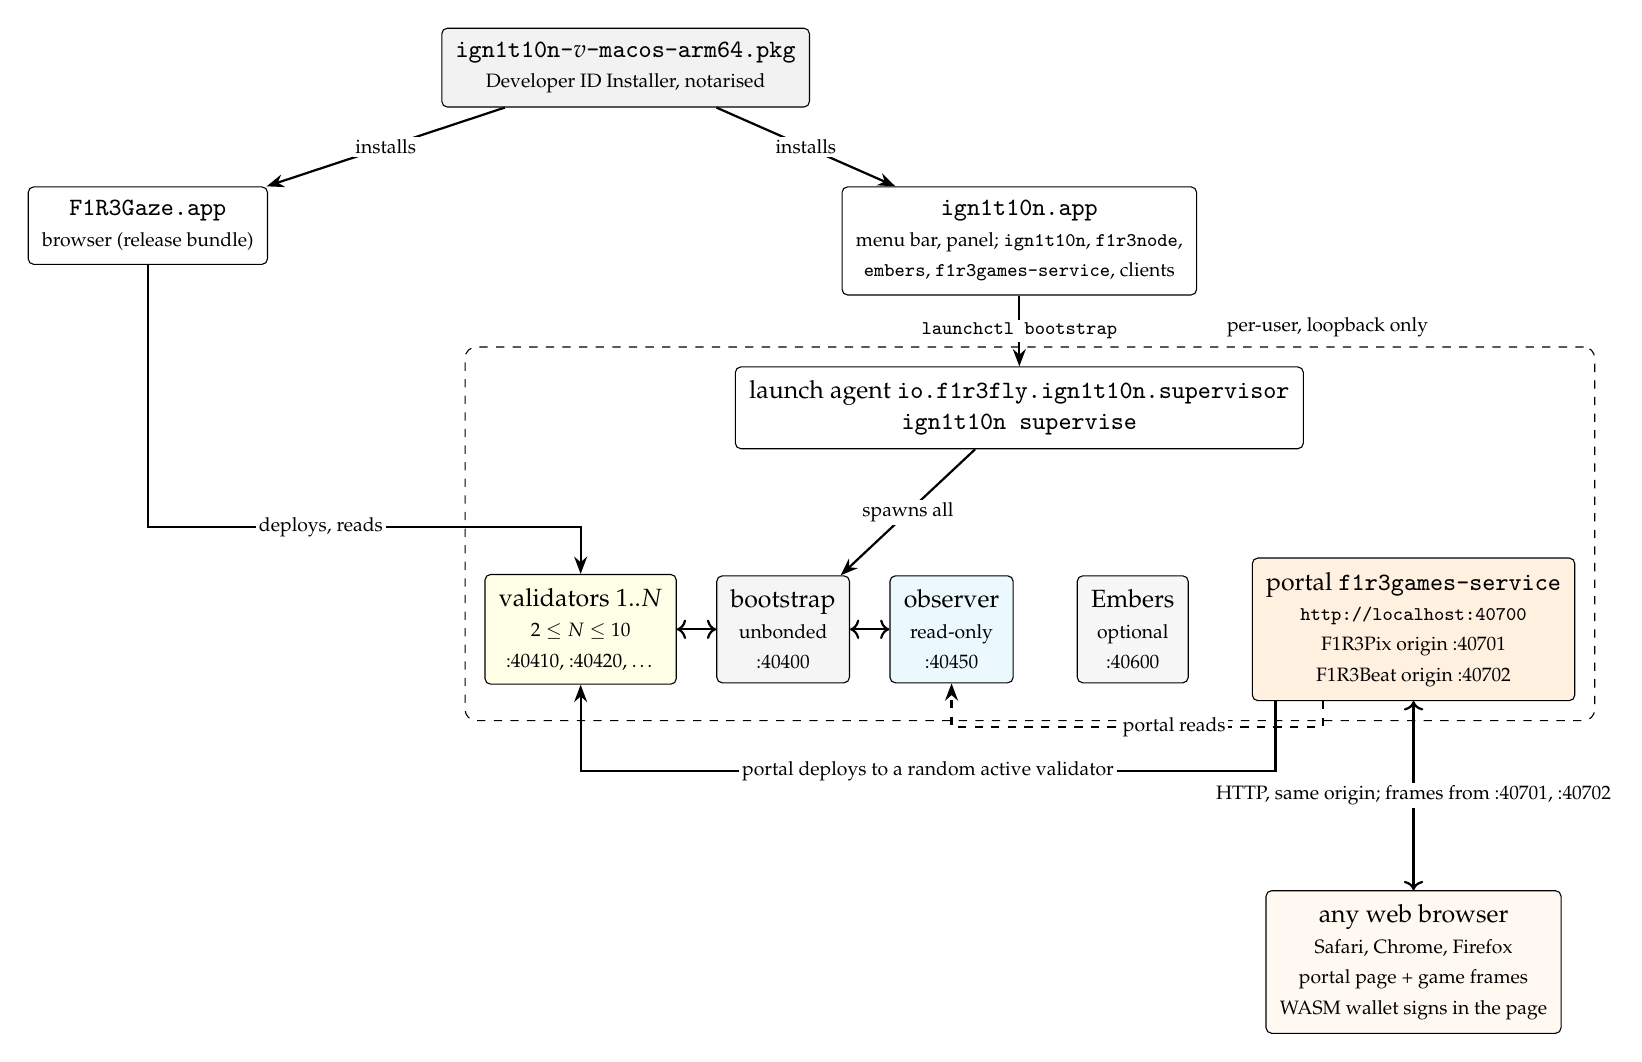
\begin{tikzpicture}[
  box/.style={draw, rounded corners=2pt, align=center, font=\small, inner sep=5pt, minimum height=9mm},
  grp/.style={draw, dashed, rounded corners=4pt, inner sep=7pt},
  arr/.style={-{Stealth[length=2.2mm]}, thick},
  lab/.style={font=\scriptsize, fill=white, inner sep=1pt}
]
\node[box, fill=black!5] (pkg) {\code{ign1t10n-}$v$\code{-macos-arm64.pkg}\\\scriptsize Developer ID Installer, notarised};
\node[box, below left=10mm and 22mm of pkg] (gaze) {\code{F1R3Gaze.app}\\\scriptsize browser (release bundle)};
\node[box, below right=10mm and 4mm of pkg] (ign) {\code{ign1t10n.app}\\\scriptsize menu bar, panel; \code{ign1t10n}, \code{f1r3node},\\\scriptsize \code{embers}, \code{f1r3games-service}, clients};
\draw[arr] (pkg) -- node[lab]{installs} (gaze);
\draw[arr] (pkg) -- node[lab]{installs} (ign);
\node[box, below=9mm of ign] (sup) {launch agent \code{io.f1r3fly.ign1t10n.supervisor}\\\code{ign1t10n supervise}};
\draw[arr] (ign) -- node[lab]{\code{launchctl bootstrap}} (sup);
\node[box, below=16mm of sup, xshift=-30mm, fill=black!4] (boot) {bootstrap\\\scriptsize unbonded\\\scriptsize :40400};
\node[box, left=5mm of boot, fill=yellow!10] (vs) {validators $1..N$\\\scriptsize $2\le N\le 10$\\\scriptsize :40410, :40420, \ldots};
\node[box, right=5mm of boot, fill=cyan!8] (obs) {observer\\\scriptsize read-only\\\scriptsize :40450};
\node[box, right=8mm of obs, fill=black!3] (emb) {\Em{}\\\scriptsize optional\\\scriptsize :40600};
\node[box, right=8mm of emb, fill=orange!12] (svc) {portal \code{f1r3games-service}\\\scriptsize \code{http://localhost:40700}\\\scriptsize F1R3Pix origin :40701\\\scriptsize F1R3Beat origin :40702};
\draw[arr] (sup) -- node[lab]{spawns all} (boot);
\draw[arr, <->] (boot) -- (vs);
\draw[arr, <->] (boot) -- (obs);
\node[grp, fit=(vs)(boot)(obs)(emb)(svc)(sup), label={[font=\scriptsize]above right:per-user, loopback only}] (g) {};
\node[box, below=24mm of svc, fill=orange!5] (www) {any web browser\\\scriptsize Safari, Chrome, Firefox\\\scriptsize portal page + game frames\\\scriptsize WASM wallet signs in the page};
\draw[arr, <->] (www) -- node[lab]{HTTP, same origin; frames from :40701, :40702} (svc);
\draw[arr] ($(svc.south west)+(0.3,0)$) |- node[lab, pos=0.75]{portal deploys to a random active validator} ($(vs.south)+(0,-1.1)$) -- (vs.south);
\draw[arr, dashed] ($(svc.south west)+(0.9,0)$) |- node[lab, pos=0.7]{portal reads} ($(obs.south)+(0,-0.55)$) -- (obs.south);
\draw[arr] (gaze.south) |- node[lab, pos=0.7]{deploys, reads} ($(vs.north)+(0,0.6)$) -- (vs.north);
\end{tikzpicture}}
\caption{What the installer lays down and what runs afterwards, with the defaults.
Nodes speak the peer protocol to one another through the bootstrap. The browser
reaches only the portal; the portal alone reaches the nodes.}
\label{fig:arch}
\end{figure}

\subsection{Components}

\begin{center}\small
\renewcommand{\arraystretch}{1.15}
\begin{tabularx}{\linewidth}{@{}p{3.3cm}X@{}}
\toprule
Component & Role\\
\midrule
\code{F1R3Gaze.app} & The \Gz{} release bundle, byte for byte.\\
\code{ign1t10n.app} & Menu-bar application and configuration panel; provisions, starts, stops, resizes, resets and reports on the shard and its services. Contains \code{ign1t10n} (one binary, three roles), \code{f1r3node}, \code{embers}, \code{f1r3games-service}, the \code{f1r3games} CLI, the portal shell and the game clients.\\
launch agent & \code{io.f1r3fly.ign1t10n.supervisor}; runs \code{ign1t10n supervise}, which owns every process below.\\
bootstrap, validators, observer & \code{f1r3node run}, as in version 0.3 (\S\ref{sec:start}).\\
\Em{} & Optional; deploys to one active validator, reads at the observer.\\
portal & \Svc{} \code{serve}: the \Gm{} API and shell at \code{http://localhost:40700}, and each bundled game client at an origin of its own (F2); deploys to one active validator, reads at the observer.\\
\Gm{} jobs & One-shot runs of \Svc{} for installation and registration (\S\ref{sec:gstages}) and, if enabled, the F1R3Beat breeder (\S\ref{sec:breeder}).\\
faucet & A key held by \Hr{}, never by a process, whose vault holds the undistributed genesis supply; funds joining validators, \Em{}, the portal, the local Cooperative and ``Fund a wallet''.\\
local Cooperative & A key held by \Hr{}; the address rendered into the portal environment as \code{coop\_address}; signs only \code{games.register} and \code{games.retire}.\\
\bottomrule
\end{tabularx}
\end{center}

\subsection{Principles}

Version 0.3's principles stand: per-user and unprivileged at run time; loopback
only; fresh secrets; one owner for the shard; a bonded validator runs; touch only
what was created; idempotent, resumable operations. Version 0.4 adds three.

\begin{principle}[Stable origins]\label{p:origin}
The portal's origin, \code{http://localhost:}\textit{port}, is fixed when it is first
allocated and never changes automatically: not at start, not on a port conflict, not
at reset, not at upgrade. Every browser keystore lives there (Finding~\ref{f:browserstate}).
The same holds for each game's origin, since manifests on the chain name it.
\end{principle}

\begin{principle}[The browser reaches only the portal]\label{p:nonode}
No page served by \Hr{} is given a node URL, and no node accepts a browser's request
(N5). Everything a page does on the chain goes through \Svc{}.
\end{principle}

\begin{principle}[Keys outlive chains]\label{p:keys}
The portal's environment key and the games' keys are kept across resets and
upgrades, so the environment URIs, and with them every pinned keystore and every
manifest hash, survive a new chain (Finding~\ref{f:pin}). They change only when the
person explicitly asks to rotate them.
\end{principle}

%======================================================================
\section{The distribution artifact}\label{sec:artifact}

\begin{requirement}[Product archive]
The release artifact \MUST{} be a flat product archive,
\code{ign1t10n-}$v$\code{-macos-arm64.pkg}, built with \code{productbuild} from two
component packages (\code{io.f1r3fly.f1r3gaze.pkg}, \code{io.f1r3fly.ign1t10n.pkg}),
signed with a \emph{Developer ID Installer} certificate, notarised and stapled. Each
component \MUST{} install its bundle to \code{/Applications} with bundle-version
checking on, so an installed newer \Gz{} is not downgraded.
\end{requirement}

\begin{requirement}[The post-install hook does one thing]
The \code{postinstall} script of the \Hr{} component package
(\code{io.f1r3fly.ign1t10n.pkg}) \MUST{} do nothing but open \Hr{} in the console user's session with \code{--first-run}, and \MUST{}
exit 0 even if that fails. It \MUSTNOT{} create files in the user's home, load agents
or generate keys. (Known issue at \code{46faa56}: nothing is visible between the
installer's Close and \Hr{}'s window; \Hr{} \SHOULD{} show its window before it
restarts an existing supervisor.)
\end{requirement}

\begin{requirement}[Platforms]
Apple silicon only; every Mach-O is \code{arm64}; minimum macOS 13.0 (resolved
decisions 2 and 3).
\end{requirement}

\begin{requirement}[No dynamic dependencies outside the system]
For every Mach-O in the archive, including \code{f1r3games-service} and
\code{f1r3games}, \code{otool -L} \MUST{} list only paths under \code{/usr/lib} and
\code{/System/Library}.
\end{requirement}

\begin{requirement}[No developer tools at install time]
The portal shell, its WebAssembly wallet and the game clients \MUST{} be shipped
built. Nothing on the person's Mac runs \code{npm}, \code{cargo},
\code{wasm-bindgen} or Vite.
\end{requirement}

%======================================================================
\section{\Hr{}}\label{sec:ign}

\subsection{Bundle layout}

\begin{lstlisting}
ign1t10n.app/Contents/
  Info.plist                    io.f1r3fly.ign1t10n, LSUIElement, arm64, min 13.0
  MacOS/ign1t10n                menu bar (default), `supervise`, `ctl`
  Helpers/f1r3node              f1r3node-rust `node` v0.4.46
  Helpers/embers                Embers 28e50d4
  Helpers/f1r3games-service     the F1R3Games portal service          (new)
  Helpers/f1r3games             the F1R3Games CLI (Decision 16)        (new)
  Resources/
    ign1t10n.icns, StatusTemplate.pdf     F1R3FLY.io brand kit (firefly bug)
    compat.toml                 storage formats this node can open
    versions.toml               what this release bundles (read at start)
    F1R3Gaze.app                installed by S0 if F1R3Gaze is missing
    f1r3games/                                                           (new)
      games.toml                per game: id, env version, template hashes, client present
      portal/                   web/dist: the shell, fonts, the wallet .wasm
      games/f1r3pix/            F1R3Pix/client/dist (index.html, preview/canvas.html)
      games/f1r3beat/           F1R3Beat/client/dist (index.html, preview/pattern.html, session.html)
    uninstall.sh
\end{lstlisting}

\noindent
The clients are served read-only from inside the signed bundle, so an upgrade
replaces them atomically and nothing in the state directory can alter them.

\subsection{One binary, three roles}

\code{ign1t10n} (Rust 1.91) is the menu bar and panel when run with no arguments, the
supervisor as \code{ign1t10n supervise}, and a client of the control socket as
\code{ign1t10n ctl} \textit{verb}. Version 0.4 adds the verbs \code{games on|off},
\code{games status [--json]}, \code{games reinstall}, \code{games open},
\code{games env} (prints the portal URL and the variables that point the
\code{f1r3games} CLI at it) and \code{games breeder on|off}. The control socket is
\code{run/control.sock}, one JSON object per line, peer uid checked.

\subsection{The launch agent}

A classic per-user agent, \code{\textasciitilde/Library/LaunchAgents/io.f1r3fly.ign1t10n.supervisor.plist},
naming the supervisor by absolute path and loaded with
\code{launchctl bootstrap gui/<uid>}. \Hr{} rewrites and reloads it whenever the path
or contents differ, and removes any \code{SMAppService} registration left by earlier
builds. (Adopted from \code{46faa56}: after a reinstall, launchd kept a stale
background-task entry for the \code{SMAppService} agent and never started it again.)
The agent still appears under Login Items. \code{KeepAlive} restarts only on an
unsuccessful exit; \code{ExitTimeOut} covers the ordered shutdown.

\subsection{The state directory}

\begin{lstlisting}
~/Library/Application Support/F1R3FLY/ign1t10n/     0700
  shard.toml                    the manifest (Appendix B), schema 4
  keys/  genesis/  conf/  nodes/  run/  archive/    as in version 0.3
  games/                                                                 (new)
    f1r3games.toml              the portal's configuration (Appendix A.2)
    manifests/<id>.json         each game's manifest as registered
    cli/                        F1R3GAMES_HOME for jobs that need the CLI
~/Library/Logs/F1R3FLY/ign1t10n/
  ign1t10n.log, <node>.stdout.log, embers.stdout.log
  portal.stdout.log, games-job.log                                       (new)
\end{lstlisting}

\subsection{Keys and Keychain items}

Node and faucet keys are as in version 0.3: encrypted PKCS\#8 PEMs, each with its own
random password in a Keychain item of service \code{io.f1r3fly.ign1t10n}, account
\code{pem.}\textit{name}; \Em{}'s secrets in \code{embers.secrets}. \Gm{} adds one
item, \code{games.secrets}, a JSON object holding the service key, the environment
key, the token secret, one environment key per game, the local Cooperative's key and
the breeder's key. Its access control list is \Hr{}'s designated requirement. A key
reaches a \Gm{} process only in that process's own environment, and only the keys the
process needs (\S\ref{sec:gkeys}).

%======================================================================
\section{Provisioning}\label{sec:prov}

Provisioning runs in the menu-bar process, as the user, when \code{shard.toml} is
absent or records an incomplete stage. Stages S0--S9 are version 0.3's, as
implemented; the first-run window's ``Advanced'' disclosure now offers the validator
count (default 2), ``Bundle \Em{}'' (default on), ``Install \Gm{}'' (default on) and
``Open \Gm{} when ready'' (default on).

\begin{description}[leftmargin=1.5em,style=nextline,itemsep=1pt]
\item[S0 preflight] macOS $\ge$ 13; Apple silicon; \Gz{} present (else install the
  bundled copy); memory and disk for $N_0+2$ nodes plus \Em{} and the portal
  (\S\ref{sec:budget}); the state directory creatable.
\item[S1 ports] node blocks of six as in version 0.3 (bootstrap 40400, validators
  40410--40440 then 40460--40510, observer 40450), \Em{} 40600, and, when \Gm{} is
  chosen, the portal and game ports of \S\ref{sec:gports}. A port is free only if it
  binds \emph{and} nothing answers a connection to it, on \code{127.0.0.1} and, for the
  portal and games, on \code{::1}.
\item[S2 the paying wallet] \Gz{}'s active wallet, or a new one labelled ``Local
  shard''.
\item[S3 keys] bootstrap, validators $1..N_0$, faucet; \Em{} secrets if chosen;
  \code{games.secrets} if chosen and absent (stage G1).
\item[S4 genesis files] \code{bonds.txt} with equal stakes of 1\,000;
  \code{wallets.txt}: 10\,000\,000~F1R3 to the browser's wallet, 1\,000~F1R3 to each
  validator, the rest of a 500\,000\,000~F1R3 supply to the faucet.
\item[S5 node configurations] \code{common.conf} and one file per node
  (Appendix A.1).
\item[S6 load the agent] \S\ref{sec:ign}.
\item[S7 genesis] bootstrap, then validators with \code{--genesis-validator}, then
  the observer; record the genesis hash, node version and storage format.
\item[S8 configure \Gz{}] the managed block or \code{settings.d} drop-in, with a
  randomly selected active validator.
\item[S9 open \Gz{}] after the observer is ready.
\end{description}

\noindent
When \Gm{} is chosen, the supervisor continues with stages G1--G7
(\S\ref{sec:gstages}) once the shard is \code{Running}, and the first-run window lists
them below S9. A failure in G1--G7 leaves the shard \code{Running} and \Gm{}
\code{Failed}; it never undoes S0--S9.

\subsection{Budgets}\label{sec:budget}

Targets on an M-series Mac with $N_0 = 2$: S0--S6 under 10\,s of machine time; genesis
under 120\,s; observer join under 180\,s; G1--G7 under 180\,s (six environment
deploys and two registrations, each waited to finalisation, about one block each);
whole first run under seven minutes. $M_{\min}$ and $D_{\min}$ add the measured
footprint of \Em{} and of the portal (a placeholder of 150\,MB each until T1 measures
it). Plays are stored on chain, so disk grows with play: T2 measures the growth per
published F1R3Pix canvas and F1R3Beat session across the $N+2$ data directories, and
the panel shows it.

%======================================================================
\section{Supervision}\label{sec:supervise}

\subsection{Start}\label{sec:start}
\begin{enumerate}[nosep]
\item Read \code{shard.toml}; refuse to start if the node's storage format is not in
  \code{compat.toml}; probe every recorded port; on conflict go to
  \S\ref{sec:portfail}.
\item Start the bootstrap; read its node id from its output.
\item Start every validator whose recorded state runs, in parallel; wait for each
  \code{/api/ready}.
\item Start the observer; wait for \code{/api/ready}.
\item If \Em{} is on: fund it once from the faucet; draw a random active validator;
  start it; wait for \code{/api/service/ready}.
\item Redraw \Gz{}'s validator. Report \code{Running}.
\item If \Gm{} is on: run any incomplete G-stage or upgrade step
  (\S\ref{sec:gupgrade}); draw a random active validator for the portal; start the
  portal; wait for readiness (\S\ref{sec:ghealth}). Report \Gm{} \code{Running}.
\item Resume an interrupted resize.
\end{enumerate}

\noindent
Node argument vectors (Appendix A.1 has the files they name):

\begin{lstlisting}
# every node
f1r3node run --config-file "$STATE/conf/<node>.conf" \
  --protocol-port B --discovery-port B+4 --api-port-grpc-external B+1 \
  --api-port-grpc-internal B+2 --api-port-http B+3 --api-port-admin-http B+5 \
  --network-id "$NETWORK_ID" --host 127.0.0.1 --no-upnp --allow-private-addresses \
  --native-token-name F1R3CAP --native-token-symbol F1R3 --native-token-decimals 8
# bootstrap adds
  --validator-private-key-path "$STATE/keys/bootstrap.pem" \
  --required-signatures $(max(N0-1,1)) --ceremony-master-mode --heartbeat-disabled
# validator k adds
  --bootstrap "rnode://$BOOT_ID@127.0.0.1?protocol=40400&discovery=40404" \
  --validator-private-key-path "$STATE/keys/validator-k.pem" [--genesis-validator]
# observer adds
  --bootstrap "rnode://$BOOT_ID@127.0.0.1?protocol=40400&discovery=40404" --heartbeat-disabled
\end{lstlisting}

\noindent
The portal runs as \code{f1r3games-service -c "\$STATE/games/f1r3games.toml" serve}
with the reduced environment (\code{HOME}, \code{PATH}, \code{TMPDIR}, \code{LANG})
plus its keys (\S\ref{sec:gkeys}) and \code{RUST\_LOG=info}; output goes to
\code{portal.stdout.log}.

\subsection{Health}
Every 10\,s the supervisor reads \code{/api/status} from every node, \Em{}'s readiness
and the portal's (\S\ref{sec:ghealth}). The shard's status machine is unchanged:
\code{Stopped} $\to$ \code{Starting(stage)} $\to$ \code{Running}
$\rightleftarrows$ \code{Degraded(reason)}, plus \code{Resizing(step)} and
\code{Failed(reason)}. \Gm{} has its own: \code{Off}, \code{Installing(stage)},
\code{Running}, \code{Degraded(reason)}, \code{Failed(reason)}, \code{Waiting} (the
shard is not \code{Running}). The menu shows both.

\subsection{Restarts}
A node that exits unexpectedly is restarted with exponential back-off (1, 2, 4,
\ldots, 60\,s); five unexpected exits of one node in five minutes stop the whole shard
in \code{Failed} rather than leave a bonded validator down. \Em{} and the portal are
restarted the same way, but five exits in five minutes put only that service in
\code{Failed}; the shard keeps running.

\subsection{Stop}\label{sec:shutdown}
On \code{SIGTERM}: the portal (and any \Gm{} job) and \Em{}, waiting up to 30\,s; the
observer, 30\,s; every validator at once, 60\,s; the bootstrap, 30\,s;
\code{SIGKILL} whatever remains. ``Stop shard'' stops everything but the supervisor;
uninstall and \code{Shutdown} also make it exit 0.

\subsection{Port conflicts at start}\label{sec:portfail}
If a node's or \Em{}'s recorded port is taken, that component is \code{Failed},
naming the port and its holder (\code{lsof}), and the menu offers ``Choose new
ports'' for every clashing node at once. The portal and game ports are \emph{not}
offered a silent move (Principle~\ref{p:origin}): \Gm{} goes \code{Failed} naming the
holder and asks the person to stop it. ``Move \Gm{} to a new address\ldots''
exists in the panel behind a dialog that says browser keystores at the old address
will not follow, offers to open the portal's Wallet page so each key can be exported
first, and then re-registers the games under their new origins (G6).

\subsection{Sleep and wake}
The processes run under a launch agent, so App Nap does not apply. The supervisor
holds a \code{PreventUserIdleSystemSleep} assertion only during provisioning, resizes
and G-stages.

%======================================================================
\section{Resizing the shard}\label{sec:resize}

Version 0.3's procedure stands: slots grow (keyed, funded, joining, bonding, active)
one after another and shrink (retiring, left, paid, absent) from the highest; the
node is stopped only after it has left the active set; a failed step stops at that
slot and offers Retry or Undo; ``Start a new shard with $M$ validators'' is a reset.
One addition: before a validator withdraws, \emph{every} client pointed at it is moved
to another active validator: \Gz{}'s setting, \Em{}, and now the portal, which is
restarted with the new \code{validator\_url} (a restart costs about a second;
deploys a page sent in that second fail and are retried by the page). With F7 the
portal takes the whole list and needs no restart.

%======================================================================
\section{\Gm{}}\label{sec:games}

\subsection{What runs}

\begin{center}\small
\renewcommand{\arraystretch}{1.15}
\begin{tabularx}{\linewidth}{@{}p{3.0cm}p{3.7cm}X@{}}
\toprule
Process & Command & Purpose\\
\midrule
portal & \code{f1r3games-service serve} & API and shell at \code{http://localhost:40700}; F1R3Pix at \code{http://localhost:40701}, F1R3Beat at \code{http://localhost:40702} (F2); faucet on\\
install job & \code{bootstrap}; \code{games-install} & G4, G5; upgrades\\
register job & \code{games-manifests}; \code{register-games} (F3) & G6; re-registration\\
breeder job & \code{beat-epoch} (F6) & optional, daily (\S\ref{sec:breeder})\\
\bottomrule
\end{tabularx}
\end{center}

\noindent
Only the portal is long-lived. Jobs are run by the supervisor one at a time, with the
portal's configuration, logged to \code{games-job.log}, and recorded in
\code{shard.toml} before and after, so an interrupted job is re-run (every job is
idempotent: each probes the chain before it deploys, Finding~\ref{f:order}).

\subsection{Origins and ports}\label{sec:gports}

\begin{center}\small
\renewcommand{\arraystretch}{1.1}
\begin{tabular}{@{}llll@{}}
\toprule
Origin & Port & Serves & Manifest \code{entry}\\
\midrule
portal & 40700 & \code{/api}, the shell & ---\\
F1R3Pix & 40701 & \code{/f1r3pix/} & \code{http://localhost:40701/f1r3pix/}\\
F1R3Beat & 40702 & \code{/f1r3beat/} & \code{http://localhost:40702/f1r3beat/}\\
Ink, SideChat, Skein & 40703--40705 & reserved & not yet registered\\
\bottomrule
\end{tabular}
\end{center}

\begin{requirement}[The host is \code{localhost}]
Every URL \Hr{} writes for the portal or a game (manifest entries,
\code{portal\_base\_url}, the menu's ``Open \Gm{}'', ``Copy \Gm{} address'') \MUST{}
use the host \code{localhost}. The portal \MUST{} redirect a request whose
\code{Host} is \code{127.0.0.1:}\textit{p} or \code{[::1]:}\textit{p} to
\code{http://localhost:}\textit{p} (308) and \MUST{} refuse any other \code{Host}
(421), which also defeats DNS rebinding (F4).
\end{requirement}

\begin{requirement}[Both loopback families]
The portal and every game origin \MUST{} listen on \code{127.0.0.1} and on
\code{::1} at the same port (F4); a port is allocated only if it is free on both
(Finding~\ref{f:dualstack}). Nothing listens on any other address.
\end{requirement}

\begin{requirement}[One origin per game]
Each bundled game \MUST{} be served from its own port, serving only its own
directory, with \code{Content-Security-Policy: frame-ancestors
http://localhost:40700} and \code{X-Content-Type-Options: nosniff}
(Decision~\ref{dec:pergame}). Games then share neither storage nor a
\code{postMessage} origin.
\end{requirement}

\noindent
Ports are allocated once, at G2, from the plan or else the first free decade in
41700--49990, and recorded; they are never moved except by the person
(\S\ref{sec:portfail}). The block 40700--40709 is outside the ports a developer's
\Gm{} checkout uses (8640, 5173, 5174), so a development portal and the installed one
run side by side against the same shard (Decision~\ref{dec:ports}).

\subsection{Keys}\label{sec:gkeys}

\begin{center}\small
\renewcommand{\arraystretch}{1.15}
\begin{tabularx}{\linewidth}{@{}>{\raggedright\arraybackslash}p{2.6cm}p{2.4cm}>{\raggedright\arraybackslash}X@{}}
\toprule
Key & Funded with & Given to\\
\midrule
service key & 1\,000\,000 F1R3 & portal (\code{F1R3GAMES\_SERVICE\_KEY}); install job; register job (pays)\\
environment key & --- & portal (\code{F1R3GAMES\_ENV\_KEY}); install job\\
token secret & --- & portal (\code{F1R3GAMES\_TOKEN\_SECRET})\\
game keys (5) & --- & install job and register job only (\code{F1R3GAMES\_GAME\_KEY\_<ID>}); F1R3Beat's also to the breeder job once, for \code{setBreeder}\\
local Cooperative & 1\,000 F1R3 & register job only (\code{F1R3GAMES\_COOP\_KEY})\\
breeder & 1\,000 F1R3 & breeder job only (\code{F1R3GAMES\_BREEDER\_KEY})\\
\bottomrule
\end{tabularx}
\end{center}

\noindent
All six kinds live in \code{games.secrets} and reach a process only in its
environment (F1). Until F1 lands, \Hr{} writes the key files a command needs into a
fresh \code{0700} directory under \code{run/}, passes their paths, waits until the
process reports ready (the service reads its keys once, at start), and deletes the
directory; the paths never appear in an argument vector except as file names.

\subsection{Installation on the chain}\label{sec:gstages}

Each stage is recorded in \code{shard.toml} under \code{[games.stages]} and resumes
at its first incomplete step.

\begin{description}[leftmargin=1.5em,style=nextline,itemsep=2pt]
\item[G1 secrets] Generate \code{games.secrets} if it is absent; otherwise keep it
  (Principle~\ref{p:keys}). Record the service, Cooperative and breeder addresses and
  every environment URI (\code{f1r3games-service env-uri} and the game-key
  derivation).
\item[G2 ports] Allocate the portal's and the bundled games' ports
  (\S\ref{sec:gports}) unless already recorded.
\item[G3 fund] Faucet transfers to the service key, the local Cooperative and (if
  the breeder is on) the breeder; wait until each is finalised at the observer.
  Skipped for an address whose balance already covers its amount.
\item[G4 configure and install the portal environment] Render
  \code{games/f1r3games.toml} (Appendix A.2) with a randomly selected active
  validator; run the install job's \code{bootstrap}; wait until the \code{env.probe}
  template at the observer reports \code{env\_version} (F5's
  \code{status --json} reports it directly).
\item[G5 install the game environments] \code{games-install --version V} with the
  versions from \code{Resources/f1r3games/games.toml}; wait until each game's probe
  reports its version. All five environments are installed, so registering a game
  whose client arrives later needs no deploy but the registration.
\item[G6 register] For each game whose client is bundled: render its manifest with
  its own origin as entry (F3, or one \code{games-manifests} run per game until F3);
  compare with \code{manifests/<id>.json} and with \code{GET /api/games/<id>}; if the
  game is absent or its template hashes or entry differ, sign \code{games.register}
  with the local Cooperative's key and wait until \code{/api/games} lists it with the
  same hashes. Save the manifest.
\item[G7 open] Start the portal (\S\ref{sec:start}); when it is ready and the person
  chose ``Open \Gm{} when ready'' at first run, \code{open http://localhost:40700/}
  in the default browser. Only at first run; later starts open nothing.
\end{description}

\subsection{Health}\label{sec:ghealth}

The portal is \emph{ready} when \code{GET /api/ready} (F5) answers 200, meaning: the
node is reachable, the registered portal environment version equals the configured
one, and every game recorded as registered is listed with the recorded hashes. Until
F5, the supervisor checks \code{GET /api/env} (the URI equals the recorded one) and
\code{GET /api/games} (each recorded game present). \Gm{} is \code{Degraded} when the
portal is ready but the observer trails or a game's hashes differ from the bundle's
(an upgrade is pending), and \code{Waiting} whenever the shard is not \code{Running}.

\subsection{What the person does in the browser}\label{sec:journey}

\begin{enumerate}[nosep]
\item \code{http://localhost:40700/}: the feed. ``Sign on'' creates a keystore
  protected by a passphrase, and optionally a passkey, or imports a key file (the
  portable format \Gz{} and F1R3Sky use, so the person's \Gz{} wallet key can be
  brought in). The page pins the portal environment URI and asks the faucet to fund
  the new address with 100~F1R3 (Decision~\ref{dec:faucet}).
\item \code{/games}: F1R3Pix and F1R3Beat, from \code{games.register}.
\item \code{/games/:id/launch}: a new instance, unlisted by default, with the game's
  configuration (F1R3Pix: capacity 61, random seating; F1R3Beat: 4/4, two bars,
  sixteenths, capacity 32, 100\,bpm). The launch sets an allowance so moves are signed
  without a prompt; payments are always prompted.
\item \code{/instances/:id}: the lobby; invite (a link at \code{localhost}, useful to
  other browsers and other accounts on this Mac), start, play in the framed client.
\item \code{/games/:id/gallery}: plays by kind and day, each previewed by the game's
  renderer from the game's own origin; \code{/plays/:id} opens one.
\end{enumerate}

\noindent
\Hr{} touches none of this; it guarantees only that the portal, its origins, the
environments and the registrations are there.

\subsection{The F1R3Beat breeder (optional)}\label{sec:breeder}

F1R3Beat's patterns breed in epochs run by a breeder key that F1R3Beat's environment
key has named (F1R3Beat design v2 \S10). When ``Run the F1R3Beat breeder daily'' is
on (Decision~\ref{dec:breeder}), \Hr{} once signs \code{setBreeder} with F1R3Beat's
game key, launches a public nursery instance with the breeder's key, records its id,
and then runs the breeder job (\code{beat-epoch}, F6) once a day while the shard runs,
skipping an epoch when nothing has been published since the last.

\subsection{Upgrade}\label{sec:gupgrade}

At start, the supervisor compares \code{Resources/f1r3games/games.toml} with what
\code{shard.toml} records:

\begin{itemize}[nosep]
\item a client-only change: nothing to do; the new bundle's files are served;
\item a game's template hashes or environment version changed: run G5 for that game
  at the recorded version $+1$ and G6, \emph{after consent}, since its live instances
  are replaced (Finding~\ref{f:upgrade}); until then the game stays registered at the
  old hashes and \Gm{} is \code{Degraded} (``F1R3Beat update waiting'');
\item the portal environment's version rose: the same, with a dialog saying that
  profiles, instances, plays, invitations and sponsorships on the local shard will be
  discarded; browser keystores are unaffected (the URI is unchanged).
\end{itemize}

\subsection{The \Gz{} rendition}\label{sec:gazerendition}

The shell's \code{core/} layer is framework-free and talks to the world through eight
capabilities, so that a f1r3lang page in \Gz{} can do the same
(\code{docs/GAZE-MAPPING.md}). When \Gz{} gains those capabilities, \Hr{} will point
\Gz{} at the portal's site (\code{f1r3://f1r3fly/games}) as well; nothing on the chain
changes. Until then the menu opens the portal in the default browser and \Gz{} in its
own window, and the two are independent.

%======================================================================
\section{User interface}\label{sec:ui}

\subsection{Menu bar}
A monochrome template image of the F1R3FLY.io firefly with a status dot: none for
\code{Running}, amber for \code{Starting}, \code{Resizing}, \code{Degraded} and
\Gm{} \code{Installing}, red for \code{Failed}, hollow for \code{Stopped}.

\begin{center}\small
\begin{tabularx}{\linewidth}{@{}p{5.0cm}X@{}}
\toprule
Item & Action\\
\midrule
\textit{Local shard: Running, 2 validators} & submenu: height, per-node readiness, observer lag, disk\\
\textit{F1R3Games: Running, 2 games} & submenu: portal address, each game and its origin, last job, breeder\\
Open F1R3Games & \code{open http://localhost:40700/} in the default browser\\
Open F1R3Gaze & \code{open -b io.f1r3fly.f1r3gaze}\\
Start / Stop shard & through the control socket\\
Configure\ldots\ (Command-comma) & the configuration panel\\
Fund a wallet\ldots & faucet transfer to any address (a \Gz{} or portal key)\\
Copy endpoints & validators, observer, shard id, \Em{}, portal\\
Show logs & reveals \code{\textasciitilde/Library/Logs/F1R3FLY/ign1t10n}\\
Reset shard\ldots{} / Uninstall\ldots & \S\ref{sec:lifecycle}\\
Quit ign1t10n & quits the menu bar only\\
\bottomrule
\end{tabularx}
\end{center}

\subsection{The configuration panel}\label{sec:panel}

The \textbf{Shard} and \textbf{General} panes are version 0.3's (validator stepper
with footprint and measured tolerance, node table, Apply sheet; run at login, use the
local shard in \Gz{}, ports, genesis amounts, \Em{} on/off). A third pane is new.

\paragraph{\Gm{}.}
\begin{itemize}[nosep]
\item \textbf{Install \Gm{}} on/off (\code{ctl games on|off}). Off stops the portal
  and frees its ports; it leaves the environments and registrations on the chain and
  the keys in the Keychain, so turning it on again needs no deploy.
\item \textbf{Address}: \code{http://localhost:40700}, read-only, with ``Open'' and
  ``Copy''; ``Move to a new address\ldots'' behind the dialog of \S\ref{sec:portfail}.
\item \textbf{Games}: one row per game: origin, environment version, registered or
  not, client bundled or not, pending update with ``Update\ldots''.
\item \textbf{Faucet amount} for new portal keys (default 100~F1R3).
\item \textbf{Run the F1R3Beat breeder daily} (default off) with the last epoch.
\item \textbf{Reinstall} (re-runs G3--G6; nothing is deployed that is already there)
  and \textbf{Rotate \Gm{} keys\ldots} (danger: new environment URIs; every browser
  keystore must be cleared, every game re-registered).
\end{itemize}

\subsection{First-run window}
F1R3FLY.io brand on a white surface (white-background logo; yellow and sky only as
rules and progress), listing S0--S9 and then G1--G7, each with a spinner, check or
error, and the ``Advanced'' disclosure of \S\ref{sec:prov}. It closes with a summary:
shard id, validators, the funded \Gz{} wallet, the portal address with an
``Open \Gm{}'' button, and where the logs are.

%======================================================================
\section{Required changes}\label{sec:wp}

\subsection{\Gz{}}
G1 (porcelain wallet commands), G2 (balances without \Em{}), G3 (\code{settings.d}),
G4 (a validator list, one drawn per deploy) and G5 (a shard health page) are
version 0.3's and \code{IMPLEMENTATION.md}'s, unchanged.

\subsection{\Nd{}}
N1 (bind addresses for transport and discovery), N2 (vendored OpenSSL and a macOS
CI build), N3 (the loopback shard test with grow and shrink), N4 (storage-format
number) and N5 (\code{api-server.reject-foreign-origin}) are unchanged
(\code{docs/node-work-packages.md}). N5 does not conflict with \Gm{}
(Finding~\ref{f:nonode}).

\subsection{\Gm{}}\label{sec:fwp}

\begin{workpackage}[F1: keys from the environment]\label{wp:f1}
\Svc{} reads \code{F1R3GAMES\_SERVICE\_KEY}, \code{F1R3GAMES\_ENV\_KEY},
\code{F1R3GAMES\_TOKEN\_SECRET}, \code{F1R3GAMES\_GAME\_KEY\_<ID>},
\code{F1R3GAMES\_COOP\_KEY} and \code{F1R3GAMES\_BREEDER\_KEY} (hex) when set, before
the configured files, and never logs them. Estimate: 0.25 engineer-week.
\end{workpackage}

\begin{workpackage}[F2: game origins served by the service]\label{wp:f2}
A repeated \code{[[origins]]} table: \code{id}, \code{listen} (a list), \code{dir};
each serves only \code{/<id>/} from \code{dir} (index fallback within it, no
directory listing) with the headers of \S\ref{sec:gports}, on its own listeners in
the same process. Estimate: 1 engineer-week.
\end{workpackage}

\begin{workpackage}[F3: headless registration and per-game entries]\label{wp:f3}
\code{games-manifests --entry ID=URL} (repeatable; \code{--entry-base} stays the
default) and \code{f1r3games-service register-games FILE [--only ID]}, which signs
\code{games.register} with \code{F1R3GAMES\_COOP\_KEY}, refuses when its address is not
the environment's \code{coop\_address}, skips a game already registered with the same
manifest, and waits for finalisation. Estimate: 0.5 engineer-week.
\end{workpackage}

\begin{workpackage}[F4: dual-stack listeners and a \code{Host} allow-list]\label{wp:f4}
\code{listen} accepts a list; the default becomes
\code{["127.0.0.1:P", "[::1]:P"]}. A configured \code{public\_host}
(\code{localhost:40700}) is the only \code{Host} served; loopback literals are
redirected to it; anything else gets 421. The same for each \code{[[origins]]}
entry. Estimate: 0.5 engineer-week.
\end{workpackage}

\begin{workpackage}[F5: readiness and status]\label{wp:f5}
\code{GET /api/ready} (\S\ref{sec:ghealth}) and \code{f1r3games-service status
--json}: the portal environment's registered version, each game environment's, and
each registered manifest's id, entry and template hashes. Estimate: 0.5
engineer-week.
\end{workpackage}

\begin{workpackage}[F6: a headless breeder (optional)]\label{wp:f6}
\code{f1r3games-service beat-set-breeder} and \code{beat-epoch --nursery ID}, signing
with the keys of F1, computing the epoch as \code{f1r3games beat epoch} does.
Estimate: 0.5 engineer-week.
\end{workpackage}

\begin{workpackage}[F7: several validators (optional)]\label{wp:f7}
\code{validator\_urls}, one drawn per deploy, with a retry on another when one
refuses, so the portal survives a validator's restart and needs no restart when one
withdraws. Estimate: 0.25 engineer-week.
\end{workpackage}

%======================================================================
\section{Security model}\label{sec:security}

\begin{center}\small
\renewcommand{\arraystretch}{1.15}
\begin{tabularx}{\linewidth}{@{}p{3.5cm}X@{}}
\toprule
Threat & Protection\\
\midrule
Reuse of public development keys & All keys generated on the Mac; the release pipeline fails if any public key from \code{docker/.env.example} or any address from \Gm{}'s \code{examples/local-shard/} appears in an artifact or in \code{shard.toml}.\\
Another user on the Mac & State directory \code{0700}; no key in any argument vector; passwords and \Gm{} keys only in the Keychain and in the owning process's environment; control socket checks the peer uid. Loopback is shared between accounts: another user can open the portal and play, as any player can, and use its faucet; the faucet is the cost.\\
Hosts on the same network & Every listener on loopback (N1, \code{api-server.host}, F4).\\
Pages in other browsers or tabs & Cannot use a node (N5). Can reach the portal's API only cross-origin: no CORS origin is configured, so responses are unreadable and JSON \code{POST}s are refused at preflight. DNS rebinding is refused by the \code{Host} allow-list (F4).\\
A malicious or buggy game & Own origin and sandbox; the host answers only that frame and that origin; the wallet signs only the game's registered play templates within the launch allowance, refuses fund-moving templates from a game, and prompts for payments (\Gm{} design).\\
Theft of a browser keystore & Encrypted under the passphrase (PBKDF2) or the passkey's PRF output; it never leaves the browser profile; \Hr{} never reads it.\\
The local Cooperative key & Governs only the registry of this local shard; it is never given to the portal process.\\
Tampered artifact & Developer ID signatures on every Mach-O and the archive; notarisation; hardened runtime with no entitlements; clients served from inside the signed bundle; GPG-signed \code{SHA256SUMS}.\\
Malware running as the user & Not defended.\\
\bottomrule
\end{tabularx}
\end{center}

%======================================================================
\section{Upgrade, reset and uninstall}\label{sec:lifecycle}

\subsection{Upgrade}
A newer archive replaces both bundles. The supervisor compares the node's storage
format (N4) with the recorded one and restarts every node on its data, or offers a new
shard; then it runs \S\ref{sec:gupgrade} for \Gm{}.

\subsection{Reset}\label{sec:reset}
``Reset shard\ldots'' archives the chain, node keys and configurations and
re-provisions from S1 with the chosen $N_0$. \code{games.secrets} is kept, so the
environment URIs are the same; G3--G6 run again on the new chain, and the portal's
origin is the same. The dialog says that every deploy, registry entry, balance,
profile, instance, play and gallery on the local shard will be gone; that \Gz{}
wallets and browser keystores keep their keys and can sign on again at once; and that
the faucet will fund them again. A checkbox ``Also rotate the \Gm{} keys'' (off) does
what the panel's rotation does.

\subsection{Uninstall}\label{sec:uninstall}
Stop everything; unload and remove the agent; after a second confirmation remove the
state directory (optionally keeping \code{archive/}), the logs and every Keychain
item of service \code{io.f1r3fly.ign1t10n} (including \code{games.secrets}); remove
\Gz{}'s managed block or drop-in; move \code{ign1t10n.app} to the Trash;
\code{pkgutil --forget io.f1r3fly.ign1t10n.pkg}. \Gz{} and its wallets are left
alone. \Hr{} cannot reach browser storage: the dialog says that keystores remain in
each browser under \code{localhost:40700} until the person clears that site's data,
and offers to open the portal's Wallet page first so keys can be exported.

%======================================================================
\section{Build and release pipeline}\label{sec:pipeline}

\code{versions.toml} gains a section, read by the release workflow and copied into
the bundle:

\begin{lstlisting}[language=Conf]
[f1r3games]
repository = "https://github.com/F1R3FLY-io/F1R3Games"
revision   = "57a3b2796108f90dd4689abf33659a34c351d2ef"   # branch f1r3beat; main once merged
toolchain  = "stable"                                      # Rust >= 1.85
node       = "22"                                          # npm ci for web/ and the clients
clients    = ["f1r3pix", "f1r3beat"]                       # Decision 11
# F1R3Games work packages this revision contains (F1..F7).
has = []
\end{lstlisting}

\begin{center}\small
\renewcommand{\arraystretch}{1.15}
\begin{tabularx}{\linewidth}{@{}p{2.0cm}p{1.9cm}X@{}}
\toprule
Job & Runner & Steps\\
\midrule
\code{node} & \code{macos-14} & \Nd{} at the pinned revision, \code{--features crypto/vendored-openssl}, arm64; \code{otool -L} gate\\
\code{embers} & \code{macos-14} & \Em{} at the pinned revision, arm64\\
\code{gaze} & \code{ubuntu} & download and verify the pinned \Gz{} release\\
\code{games} (new) & \code{macos-14} & \Gm{} at the pinned revision: \code{cargo test} for the workspace and \code{rholint}; \code{cargo build --release -p f1r3games-service -p f1r3games-cli}, arm64; \code{web/}: \code{npm ci}, build the wallet to WebAssembly (\code{wasm32-unknown-unknown}, \code{wasm-bindgen} 0.2.129), \code{npm test}, \code{npm run build}; each listed client: \code{npm ci}, \code{npm test}, \code{npm run build}; write \code{games.toml} (environment versions and template hashes from \code{games-manifests}); \code{otool -L} gate\\
\code{ign1t10n} & \code{macos-14} & build, unit and end-to-end tests (the stand-in node gains a stand-in portal)\\
\code{assemble} & \code{macos-14} & \code{build.sh} with the \Gm{} artifacts; sign inside out (\code{Helpers/*}, \code{MacOS/ign1t10n}, the app); \code{pkgbuild}, \code{productbuild}, sign, notarise, staple\\
\code{smoke} & \code{macos-14} & headless provisioning with \Gm{} on; A2--A6, A11, A12, A15, A17, A23; A16 in headless Chromium and WebKit\\
\code{publish} & \code{ubuntu} & \code{SHA256SUMS}, GPG signature; draft release\\
\bottomrule
\end{tabularx}
\end{center}

%======================================================================
\section{Testing and acceptance}\label{sec:accept}

A1--A14 are version 0.3's: clean install; round trip through \Gz{}; loopback only; no
foreign libraries; no shipped secrets; persistence across reboot; port conflict with
a Docker shard; crash recovery; upgrade; uninstall; grow in place; shrink in place;
new shard at the maximum; bounds and interruption. A1 now also requires \Gm{}
\code{Running} within seven minutes. New:

\begin{description}[leftmargin=1.5em,style=nextline,itemsep=2pt]
\item[A15 \Gm{} installed.] After A1, \code{ctl games status --json} reports the
  portal ready, six environments at their bundled versions, and F1R3Pix and F1R3Beat
  registered with entries at \code{localhost:40701} and \code{:40702}.
\item[A16 Playing in a stock browser.] Driven by Playwright in Chromium, WebKit and
  Firefox: sign on with a passphrase; the faucet funds the key; launch an F1R3Pix
  instance; seat, paint, publish a canvas; the gallery lists it and the renderer
  draws it; then the same for F1R3Beat with a pattern. Repeat sign-on with a passkey
  where the browser supports the PRF extension.
\item[A17 Origins.] \code{http://127.0.0.1:40700/} redirects to \code{localhost}; a
  request with \code{Host: evil.example} gets 421; the portal refuses to frame a game
  whose entry is its own origin; game responses carry \code{frame-ancestors}; one
  game's origin does not serve another's files.
\item[A18 Dual stack.] With a decoy listener on \code{[::1]:40700} before
  provisioning, G2 allocates another decade. With one started after provisioning,
  \Gm{} goes \code{Failed} naming the holder and does not move.
\item[A19 Reset keeps identities.] A keystore created before ``Reset shard'' signs on
  afterwards without a pin error; the environment URIs are unchanged; G3--G6 ran.
\item[A20 Upgrades.] A bundle whose only change is a client deploys nothing; one with
  a changed F1R3Beat template asks consent, installs version $+1$ and re-registers;
  F1R3Pix is untouched.
\item[A21 Evacuation.] Shrinking away the portal's validator moves the portal first;
  a move sent during the shrink finalises.
\item[A22 Off and on.] \code{ctl games off} frees ports 40700--40702; \code{on}
  restarts with no deploy and the same origin.
\item[A23 Loopback.] \code{lsof} lists \code{f1r3games-service} only on
  \code{127.0.0.1} and \code{::1}.
\end{description}

%======================================================================
\section{Work packages and schedule}\label{sec:plan}

\begin{center}\small
\renewcommand{\arraystretch}{1.15}
\begin{tabularx}{\linewidth}{@{}>{\raggedright\arraybackslash}p{1.3cm}X p{0.9cm}>{\raggedright\arraybackslash}p{2.2cm}@{}}
\toprule
WP & Deliverable & Est. & Status\\
\midrule
N1--N5 & node: bind addresses, macOS build, loopback shard test, storage format, origin guard & 4.5 & open\\
G1--G5 & \Gz{}: porcelain, balances, \code{settings.d}, validator list, health page & 2.5 & open\\
H1--H6 & \Hr{}: provisioning, supervision, UI, resize, panel, lifecycle & 11 & first working version\\
R1, T1 & release workflow; acceptance and measurements & 3.5 & partly\\
\midrule
F1--F5 & \Gm{}: keys from environment, game origins, headless registration, dual stack and \code{Host}, readiness & 2.75 & new\\
F6, F7 & \Gm{}: headless breeder; validator list (optional) & 0.75 & new\\
H7 & \Hr{}: manifest schema 4, \code{games.secrets}, stages G1--G7, the portal role, jobs, health, evacuation, upgrade comparison & 2.5 & new\\
H8 & \Hr{}: menu items, \Gm{} pane, first-run additions, opening the browser & 1 & new\\
H9 & \Hr{}: reset, rotation, uninstall and upgrade dialogs for \Gm{} & 1 & new\\
R2 & release: the \code{games} job, bundle layout, signing, smoke additions & 1 & new\\
T2 & A15--A23; browser matrix; footprint and on-chain growth of plays & 1.5 & new\\
\bottomrule
\end{tabularx}
\end{center}

\noindent
The new work is about 10.5 engineer-weeks. F2, F3 and F5 are on its critical path:
H7 needs game origins to register entries, headless registration to finish G6, and
readiness to supervise. F1 and F4 can follow (H7 has an interim for F1). With one
engineer on \Gm{} (F1--F7) and one on \Hr{} (H7--H9, R2), and T2 shared, the
component fits in five to six calendar weeks, alongside the open version 0.3 work.

%======================================================================
\section{Obligations and decisions}\label{sec:open}

\subsection{Obligations}

Version 0.3's obligations stand: the loopback shard works (N3); resizing works (N3);
footprint (T1); measured fault tolerance (T1); PEM compatibility (discharged at
\code{46faa56}). Added:

\begin{obligation}[The environments behave on a node]\label{ob:envs}
Before H7 is merged, T2 must show, on an \Hr{} shard at the pinned node, the portal
environment and the F1R3Pix and F1R3Beat environments doing what their designs say,
including the parts \Gm{}'s \code{IMPLEMENTATION.md} lists as unverified (the
\code{TreeHashMap} handle, sponsorship escrow, \code{/\textbackslash\ Int} and
\code{/\textbackslash\ String} patterns, phlo per move), and record phlo per move and
per read so the allowance and capacity defaults rest on measurements.
\end{obligation}

\begin{obligation}[Browsers]\label{ob:browsers}
T2 must establish, for current Safari, Chrome and Firefox on macOS 13--26: that
\code{http://localhost} is a secure context for WebAuthn, IndexedDB and WebAssembly;
which support the PRF extension the passkey unlock needs (the passphrase works in
all); and that the sandboxed game frames with \code{allow-same-origin} exchange
messages with the portal. The first-run summary names any browser found wanting.
\end{obligation}

\begin{obligation}[Origin stability]\label{ob:origin}
The end-to-end test must show that no path through start, port conflict, resize,
reset, upgrade or \Gm{} off/on changes a recorded \Gm{} port.
\end{obligation}

\begin{obligation}[\Em{} compatibility]\label{ob:embers}
\Em{} \code{28e50d4}'s contracts do not parse at node \code{fce422a}. \Gm{} does not
depend on \Em{}, but the release must not ship a pair that fails: pin a compatible
\Em{} or default \Em{} off, and make the smoke job deploy its contracts.
\end{obligation}

\subsection{Resolved on 30 September 2026}\label{sec:resolved}

\begin{center}\small
\renewcommand{\arraystretch}{1.12}
\begin{tabularx}{\linewidth}{@{}p{0.6cm}p{3.6cm}X@{}}
\toprule
\# & Decision & Resolution\\
\midrule
1 & Fold the bootstrap into validator~1 & No: keep the separate bootstrap for version 1.\\
2 & Intel & Apple silicon only.\\
3 & Minimum macOS & 13.0.\\
4 & Genesis amounts & 10\,000\,000~F1R3 to the browser's wallet; validators 1\,000~F1R3 fees and 1\,000 stake; the rest of 500\,000\,000 to the faucet.\\
5 & Where deploys go & A randomly selected active validator, redrawn at each start and after each resize; with G4, the whole list.\\
6 & Timings & Tuned for a laptop (profile \code{laptop-v1}: casper loop 1.0\,s at $N=2$ rising to 3.0\,s at $N=10$; heartbeat on; maximum LFB age 15\,s, or 30\,s above $N=4$); recalibrated by T1.\\
7 & Foreign \code{Origin} & The node refuses it (N5).\\
8 & \Em{} & An installation option, default on.\\
\bottomrule
\end{tabularx}
\end{center}

\subsection{Open decisions}

\setcounter{decision}{8}
\begin{decision}[The \Gm{} port block]\label{dec:ports}
40700--40709, beside \Hr{}'s other blocks and apart from a developer's 8640, 5173 and
5174 (proposed); or the service's own default, 8640, which would collide with a
development portal.
\end{decision}

\begin{decision}[Who is the Cooperative on the local shard]\label{dec:coop}
A key \Hr{} generates and holds (proposed): registration then needs nothing from the
person, and the key governs nothing outside this shard. Or the person's own key,
imported, so that the same identity governs every shard they run.
\end{decision}

\begin{decision}[Which games to register]\label{dec:which}
Install all five environments; register only games whose web client is bundled,
F1R3Pix and F1R3Beat (proposed), adding the others as clients land. Or register all
five now, which lists three games the browser cannot play.
\end{decision}

\begin{decision}[One origin per game]\label{dec:pergame}
Per-game origins (proposed), as the portal's isolation model intends; or one shared
games origin, which is simpler but lets games read one another's storage.
\end{decision}

\begin{decision}[Opening the browser]\label{dec:open}
At the end of first run, open the portal in the default browser as well as \Gz{}
(proposed); or show only the ``Open \Gm{}'' button.
\end{decision}

\begin{decision}[Faucet amount]\label{dec:faucet}
100~F1R3 per new portal key on the local shard (proposed), enough for allowances and
F1R3Pix and F1R3Beat payments between players; or the service default of 1~F1R3.
\end{decision}

\begin{decision}[The F1R3Beat breeder]\label{dec:breeder}
Off by default, a switch in the panel (proposed), since a single person's local shard
produces little engagement to select on; or on, daily.
\end{decision}

\begin{decision}[Ship the CLI]\label{dec:cli}
Bundle \code{f1r3games} in \code{Helpers} with \code{ctl games env} printing how to
point it at the local portal (proposed); it is how a developer scripts plays and runs
\code{beat verify}.
\end{decision}

\begin{decision}[\Gm{} by default]\label{dec:default}
On by default in the first-run window, like \Em{} (proposed).
\end{decision}

%======================================================================
\appendix
\section{Configuration templates}\label{app:conf}

\subsection*{A.1 Node configuration}

\code{conf/common.conf}, \code{bootstrap.conf}, \code{validator-\{k\}.conf} and
\code{observer.conf} are version 0.3's, with the \code{laptop-v1} timing values in
place of \code{docker/conf/default.conf}'s and \code{logging.sink = "stdout"}:

\begin{lstlisting}[language=Hocon]
# conf/common.conf (excerpt): rendered by ign1t10n; values for N validators
protocol-server { network-id = "{{NETWORK_ID}}", bind-address = "127.0.0.1",  # N1
                  allow-private-addresses = true, no-upnp = true }
protocol-client.network-id = "{{NETWORK_ID}}"
peers-discovery { bind-address = "127.0.0.1", lookup-interval = 60 seconds }
api-server { host = "127.0.0.1", reject-foreign-origin = true }                # N5
casper {
  shard-name = "root"
  fault-tolerance-threshold = 0.1
  casper-loop-interval = {{LOOP_MS}} ms        # 1000 at N = 2 .. 3000 at N = 10
  heartbeat { enabled = true, max-lfb-age = {{LFB_AGE}} seconds }
  genesis-ceremony { required-signatures = {{max(N0-1,1)}},
                     approve-interval = 10 seconds, approve-duration = 1 minutes }
  genesis-block-data { bonds-file = "{{STATE}}/genesis/bonds.txt",
                       wallets-file = "{{STATE}}/genesis/wallets.txt",
                       number-of-active-validators = 10,
                       epoch-length = 10, quarantine-length = 10 }
}
logging { format = "json", sink = "stdout" }
\end{lstlisting}

\subsection*{A.2 \code{games/f1r3games.toml}}

\begin{lstlisting}[language=Conf]
# Rendered by ign1t10n at G4 and at every start (the validator is redrawn).
listen        = ["127.0.0.1:40700", "[::1]:40700"]      # F4; one address until it lands
public_host   = "localhost:40700"                       # F4
shard_id      = "root"
validator_url = "http://127.0.0.1:40420"                # a randomly drawn active validator
observer_url  = "http://127.0.0.1:40453"
coop_address  = "{{LOCAL_COOPERATIVE_ADDRESS}}"
env_version   = 1                                       # from Resources/f1r3games/games.toml
phlo_price    = 1
default_phlo_limit = 500000
max_phlo_limit     = 50000000
env_phlo_limit     = 50000000
deploy_ttl_ms      = 600000
token_ttl_secs     = 3600
bootstrap_env      = false        # installation is a job (G4), not a side effect of serve
cors_origins       = []           # the shell is same-origin
portal_base_url    = "http://localhost:40700"
static_dir         = "/Applications/ign1t10n.app/Contents/Resources/f1r3games/portal"
# keys come from the environment (F1); until then, *_file paths in a 0700 run directory

[faucet]
enabled = true
amount  = 10000000000             # 100 F1R3 (Decision 14)

[[origins]]                       # F2
id     = "f1r3pix"
listen = ["127.0.0.1:40701", "[::1]:40701"]
public_host = "localhost:40701"
dir    = "/Applications/ign1t10n.app/Contents/Resources/f1r3games/games"

[[origins]]
id     = "f1r3beat"
listen = ["127.0.0.1:40702", "[::1]:40702"]
public_host = "localhost:40702"
dir    = "/Applications/ign1t10n.app/Contents/Resources/f1r3games/games"
\end{lstlisting}

\section{The manifest}\label{app:manifest}

Schema 4 adds \code{[options].games}, \code{[options].games\_open\_at\_first\_run}
and the \code{[games]} tables to schema 3; an absent \code{[games]} reads as
\Gm{} never installed, so a schema-3 manifest upgrades in place.

\begin{lstlisting}[language=Conf]
# ~/Library/Application Support/F1R3FLY/ign1t10n/shard.toml (excerpt)
schema = 4

[options]
embers = true
gaze_integration = true
deploy_target = "random"
timing = "laptop-v1"
games = true
games_open_at_first_run = true

[games]
revision = "57a3b27"                     # the F1R3Games revision last installed
portal_port = 40700
validator_slot = 2                       # drawn at each start
service_address = "1111...Xs"
coop_address = "1111...Cp"
breeder_address = "1111...Br"
env_uri = "rho:id:...g7"
env_version = 1
faucet_f1r3 = 100
breeder = false

[[games.game]]
id = "f1r3pix"
port = 40701
env_uri = "rho:id:i77c...gtgn"
env_version = 2
client = true
registered = true
manifest_sha256 = "5e0c...91"

[[games.game]]
id = "f1r3beat"
port = 40702
env_uri = "rho:id:...q4"
env_version = 1
client = true
registered = true
manifest_sha256 = "a3b1...0d"

[[games.game]]
id = "f1r3ink"                           # environment installed, not registered
env_uri = "rho:id:...k2"
env_version = 1
client = false
registered = false

[games.stages]                           # G1..G7, cleared from G3 at reset
secrets = true
ports = true
funded = true
portal_env = true
game_envs = true
registered = true
opened = true

[games.job]                              # present only while a job runs
kind = "register"
game = "f1r3beat"
started = 2026-10-14T09:20:03Z
deploy = "3045...aa"
\end{lstlisting}

\end{document}
